
\section {Predictions of single $\mu$-like ring event reconstructed energy spectrum in SuperK}
\label{sec:spectrum_prediction}

\subsection {Methodology}

In this analysis, 
the oscillation parameters are determined 
by fitting the reconstructed energy ($E_{r}$) spectrum
of 1-ring $\mu$-like events observed at SuperK with the predicted spectrum.
The predicted number $N_{SK;r}$ 
of 1-ring $\mu$-like events in the $r^{th}$ reconstructed energy bin
is computed as follows:

\begin{equation}
\displaystyle
  N_{SK;r} = 
    \sum_{m} \sum_{t} \sum_{r\prime}
        P_{m;t} \cdot
        T_{r;r\prime;f_{{\Delta}E}} \cdot
        S_{m;t;r\prime;\vec{f}} \cdot
        N_{SK;m;r\prime;t}^{MC} \cdot
\label{eq:far_prediction}
\end{equation}

In Eq.\ \ref{eq:far_prediction}, $N_{SK;m;r\prime;t}^{MC}$ is the input SuperK Monte Carlo (MC) template 
containing the number of events in the 1-ring $\mu$-like MC sample with true reaction mode $m$, 
and found in the true energy bin t and the reconstructed energy bin $r\prime$.
The construction of the nominal MC templates is discussed in Sec.\ \ref{sec:mc_templates}.
Both flux-tuning weights based on NA61 hadro-production data (see Sec.\ \ref{sec:na61_weights})
and flux and cross-section tuning weights based on ND280 data (see Sec.\ \ref{sec:banff_weights})
are applied to the nominal MC templates.
$S_{m;t;r\prime;\vec{f}}$ is an overall, multiplicative, systematic error factor 
depending on the reaction mode $m$, the true energy bin $t$, the reconstructed energy bin $r\prime$ 
and a vector of nuisance (systematic) parameters $\vec{f}$. 
A complete desciption of the nuisance parameters considered in this analysis is given in Sec. \ref{sec:systematics}.
$T_{r;r\prime;f_{{\Delta}E}}$ is a transfer function describing the migration of events
between the reconstructed energy bins $r$ and $r\prime$ due to uncertainty in the SuperK reconstructed energy
scale, expressed here in terms of the nuisance parameter $f_{{\Delta}E}$.
Finally, $P_{m;t}$ is the 3-flavour oscillation probability applied in the true energy
bin t of the SuperK MC template which corresponds to mode $m$.
Application of the term $P_{m;t}$ is discussed in Sec.\ \ref{sec:applying_oscillations}.

%....................................................................................................................
%....................................................................................................................

\subsection {Construction of nominal SuperK Monte Carlo templates}
\label{sec:mc_templates}

The nominal SuperK 1-ring $\mu$-like MC templates $N_{SK;m;r;t}^{MC}$
are constructed by applying the 1-ring $\mu$-like selection cuts to the official SuperK MC samples.
Details of the MC samples are given in Sec. \ref{sec:mc_templates:input_mc}.
The calculation of the normalization of each MC sample is described in Sec.\ \ref{sec:mc_templates:normalization}.
The official 1-ring $\mu$-like selection cuts are listed in Sec.\ \ref{sec:mc_templates:1Rmu_cuts}.
The list of MC templates used in this analysis is shown in Sec.\ \ref{sec:mc_templates:template_list},
while the true and reconstructed energy binning of the templates is discussed 
in Sec. \ref{sec:mc_templates:template_binning}.

The nominal SuperK MC templates used in this analysis are shown in Appendix \ref{appendix:mc_template_binning_studies:templates}.

%....................................................................................................................
\subsubsection {Input Monte Carlo samples}
\label{sec:mc_templates:input_mc}

This analysis uses the official 2011c SuperK MC sample \cite{SKsample},
which was generated and processed at the Kamioka cluster.
The following versions of software packages were used:
\begin{itemize}
  \item JNUBEAM flux 2011a
  \item NEUT v5.1.4.1
  \item SKDETSIM-v12p80
  \item ATMPD-ap11c
  \item SKOFL-11c
\end{itemize}

Five MC samples were generated.
Four of the samples
($\nu_{\mu}$, $\bar{\nu_{\mu}}$, $\nu_{e}$ and $\bar{\nu_{e}}$) 
were generated using the nominal JNUBEAM flux without oscillations.
A fifth sample of $\nu_{e}$ interactions was also generated with the $\nu_{\mu}$ flux.
This fifth sample will be denoted the `oscillated $\nu_{e}$' sample (it corresponds to the `signal-$\nu_{e}$' 
sample in the $\nu_{e}$-appearance analysis).
Samples neglected would make a negligible contribution to the single $\mu$-like ring sample as explained in 
the following subsections.
All samples were generated including the neutrino flux estimates up to 30 GeV.
The flux histograms used for neutrino event generation had 50 MeV bins.

%....................................................................................................................
\subsubsection {Normalization of Monte Carlo samples}
\label{sec:mc_templates:normalization}

The normalization (integrated exposure in terms of POT) of each event sample is calculated from
the number of events with a MC truth interaction vertex within the 22.5 kt fiducial volume.

\begin{equation}
\displaystyle
  N = \int  dS dI dE \cdot
            \frac{d^{3}\Phi_{SK}}{dS dI dE_{\nu}} \cdot
            \sigma_{H_{2}O} \cdot
            \frac{N_{A}}{A} \cdot \rho \cdot L 
\end{equation}
where 
$d^{3}\Phi_{SK}$/$dS dI dE$ is the number of flux particles, for the given neutrino species,
per neutrino energy bin $dE_{\nu}$, 
per unit area $dS$ 
and per POT,
$\sigma_{H_{2}O}$ is the total interaction cross section in water
for the given neutrino species,
I is the beam intensity in terms of POT,
$N_{A}$ is  Avogadro's number,
$A$ is the mass number for water,
$\rho$ is the water density
and L is the neutrino path length in the water volume.
The results of this calculation are shown in Tab.\ \ref{tab:SKMCSummary} for all 5 SuperK MC samples along with 
the generated statistics, the numbers of events within the 22.5 kt fiducial volume and the
derived POT normalization of each sample in terms of POT.

After being generated from a MC sample corresponding to a calculated integrated beam exposure I,
each MC template is normalized to the integrated beam exposure of the Run1+2+3 dataset (3.010$\times$10$^{20}$ POT)
by scaling the bin contents of the template with 3.010$\times$10$^{20}$/I.

\begin{table}
\centering
\begin{tabular}{| c | c | c | c | c |}
\hline
Sample             &  Number of events   &  Number of events  & Number of events  & POT normalization \\
                   & /22.5 kt fiducial /$10^{21}$ POT  & generated  & in fiducial volume  &               \\  
\hline             
$\nu_{\mu}$           &         1418.68           &       1000000             &          634998         &    4.4760 $\times 10^{23}$  \\
$\bar{\nu_{\mu}}$  &             48.6039        &         504000             &         319640         &    6.5762  $\times 10^{24}$ \\
$\nu_{e}$              &              28.312         &        1000000            &         633715         &     2.2383  $\times 10^{25}$ \\
$\bar{\nu_{e}}$     &                2.98885      &          504000            &         319689        &     1.0696  $\times 10^{26}$ \\
Oscillated $\nu_{e}$    
                            &             1490.15         &          504000            &         320252        &      2.1491 $\times 10^{23}$ \\
\hline
\end{tabular}
\caption{
  Statistics and normalization of input SuperK MC samples.
}
\label{tab:SKMCSummary}
\end{table}

%....................................................................................................................
\subsubsection {Single $\mu$-like ring event selection cuts}
\label{sec:mc_templates:1Rmu_cuts}

The SuperK MC templates contain events from the 
$\nu_{\mu}$, $\bar{\nu_{\mu}}$, $\nu_{e}$, $\bar{\nu_{e}}$ and oscillated $\nu_{e}$ samples
passing the standard SuperK selection cuts for 1 $\mu$-like ring events.
These cuts are:

\begin{itemize}
\item
the number of PMT hits in the highest-charge OD cluster is less than or
equal to 15, and the event passes the flasher rejection cuts
({\tt evclass == 1}),
\item
the reconstructed vertex is at least 2 metres away from the ID wall 
({\tt wall $>$ 200}),
\item
the visible energy in the event is above 30 MeV 
({\tt evis  $>$ 30}),
\item
there is exactly 1 reconstructed ring in the event 
({\tt nring == 1}),
\item
the reconstructed ring is $\mu$-like 
({\tt ip[0] = 3}),
\item
the reconstructed muon momentum is above 200 MeV 
({\tt amomm[0] $>$ 200}), and
\item
there is at most 1 decay e$^{-}$ in the event 
({\tt nmue $<$= 1}).
\end{itemize}

%....................................................................................................................
\subsubsection {List of Monte Carlo templates}
\label{sec:mc_templates:template_list}

For each SuperK MC sample, a number of different MC templates is constructed 
corresponding to different true reaction modes.
The template granularity depends on the type of oscillation analysis and the specific 
systematic parameters considered in the analysis.
12 MC templates were used for our 2010 Run1+2 2-flavour disappearance analysis \cite{OurRun12DisappAnalysis}, while
15 MC templates were used for our 2010 Run1+2 3-flavour disappearance analysis \cite{OurRun12DisappAnalysis3Flavour}.
This analysis uses the following 28 MC templates:

\begin{itemize}
\item  $\nu_{\mu}$ CCQE
\item  $\nu_{\mu}$ CC1$\pi$, 
\item  $\nu_{\mu}$ CC coherent, 
\item  $\nu_{\mu}$ CC other, 
\item  $\nu_{\mu}$ (and $\rightarrow$ $\nu_{e}$, $\nu_{\tau}$) NC1$\pi^{\pm}$, 
\item  $\nu_{\mu}$ (and $\rightarrow$ $\nu_{e}$, $\nu_{\tau}$) NC other, 
\item  $\bar{\nu}_{\mu}$ CCQE, 
\item  $\bar{\nu}_{\mu}$ CC1$\pi$, 
\item  $\bar{\nu}_{\mu}$ CC coherent, 
\item  $\bar{\nu}_{\mu}$ CC other, 
\item  $\bar{\nu}_{\mu}$(and $\rightarrow$ $\bar{\nu}_{e}$, $\bar{\nu}_{\tau}$) NC1$\pi^{\pm}$, 
\item  $\bar{\nu}_{\mu}$(and $\rightarrow$ $\bar{\nu}_{e}$, $\bar{\nu}_{\tau}$) NC other, 
\item  $\nu_{e}$ CCQE, 
\item  $\nu_{e}$ CC1$\pi$,
\item  $\nu_{e}$ CC coherent,
\item  $\nu_{e}$ CC other,
\item  $\nu_{e}$ (and $\rightarrow$ $\nu_{\mu}$, $\nu_{\tau}$) NC1$\pi^{\pm}$,
\item  $\nu_{e}$ (and $\rightarrow$ $\nu_{\mu}$, $\nu_{\tau}$) NC other,
\item  $\bar{\nu}_{e}$ CCQE, 
\item  $\bar{\nu}_{e}$ CC1$\pi$,
\item  $\bar{\nu}_{e}$ CC coherent,
\item  $\bar{\nu}_{e}$ CC other,
\item  $\bar{\nu}_{e}$ (and $\rightarrow$ $\bar{\nu}_{\mu}$, $\bar{\nu}_{\tau}$) NC1$\pi^{\pm}$,
\item  $\bar{\nu}_{e}$ (and $\rightarrow$ $\bar{\nu}_{\mu}$, $\bar{\nu}_{\tau}$) NC other,
\item  Oscillated $\nu_{e}$ CCQE, 
\item  Oscillated $\nu_{e}$ CC1$\pi$,
\item  Oscillated $\nu_{e}$ CC coherent and
\item  Oscillated $\nu_{e}$ CC other
\end{itemize}

In the standard 3-flavour oscillation framework,
oscillations of $\nu_{e}$ and $\nu_{\mu}$ can yield $\nu_{\tau}$, while
oscillations of $\bar{\nu}_{e}$ and $\bar{\nu}_{\mu}$ can yield $\bar{\nu}_{\tau}$.
In this analysis, we neglect contributions from $\nu_{\tau}$-CC and $\bar{\nu}_{\tau}$-CC as their
energy threshold is around 3.5 GeV and their effect is negligible.
Accordingly, this analysis uses no $\nu_{\tau}$-CC and $\bar{\nu}_{\tau}$-CC MC templates
(and, in fact, no $\nu_{\tau}$ and $\bar{\nu}_{\tau}$ SuperK MC samples are available).

It should be emphasized here that
the $\nu_{\mu}$ NC MC templates for a mode $m$ are proxies for the
NC MC templates for the mixture of $\nu_{e}$+$\nu_{\mu}$+$\nu_{\tau}$ resulting from 
3-flavour $\nu_{\mu}$ oscillations for that mode $m$. The same applies to the $\bar{\nu}_{\mu}$, $\nu_{e}$ and $\bar{\nu}_{e}$ NC MC templates.
These NC MC templates are unchanged under standard 3-flavour oscillations (see also Sec.\ \ref{sec:applying_oscillations}).

Also it should be noted that there are no explicit NC MC templates made from the oscillated $\nu_{e}$ sample.
If they were used, the oscillated $\nu_{e}$ (i.e.\ $\nu_{e}$ coming from $\nu_{\mu}$ oscillations) would be double counted 
since they are already included in the $\nu_{\mu}$ NC MC templates.

%....................................................................................................................
\subsubsection {Binning of Monte Carlo templates}
\label{sec:mc_templates:template_binning}

Each of the 28 MC templates has 6132 2-dimensional bins (= 84 true energy bins $\times$ 73 reconstructed energy bins).
The 84 true energy bins are arranged as follows:
\begin{itemize}
 \item   6 50-MeV bins from 0-0.3 GeV, 
 \item   28 25-MeV bins from 0.3-1 GeV, 
 \item   40 50-MeV bins from 1-3 GeV, 
 \item   5 100-MeV bin from 3-3.5 GeV, 
 \item   1 bin from 3.5-4 GeV, 
 \item   1 bin from 4-5 GeV, 
 \item   1 bin from 5-7 GeV, 
 \item   1 bin from 7-10 GeV and
 \item   1 bin from 10-30 GeV.
\end{itemize}

The 73 reconstructed energy bins are the following:
\begin{itemize}
 \item   60 50-MeV bins from 0-3 GeV, 
 \item   4 250-MeV bins from 3-4 GeV, 
 \item   4 500-MeV bins from 4-6 GeV, 
 \item   4 1000-MeV bins from 6-10 GeV and
 \item   1 bin from 10-30 GeV.
\end{itemize}
The same reconstructed neutrino energy binning is used for the fit of the 1-ring $\mu$-like reconstructed energy spectrum.

A study was performed to decide the optimum binning scheme balancing the needs for accuracy and speed.
Details are given in Appendix \ref{appendix:mc_template_binning_studies:etrue}-\ref{appendix:mc_template_binning_studies:ereco}.

%....................................................................................................................
%....................................................................................................................
\subsection {Applying flux tuning based on NA61 data}
\label{sec:na61_weights}

In this analysis, the nominal MC templates, which were constructed using a MC event sample generated with 11a flux,
are reweighted to the {\em 2011b\_v3.2\_run1-3c} flux which was tuned on NA61 hadroproduction measurements \cite{FluxTuning}\cite{NA61T2K}.
The reweighted MC templates are denoted the {\em NA61-tuned} MC templates in this document.
The applied weights, as a function of the true neutrino energy, were obtained from \cite{FluxTuningHistograms}
and are shown in Figs.\ \ref{fig:na61_weights:numu}-\ref{fig:na61_weights:nuebar}.
The effect of this flux tune on the predicted reconstructed energy spectrum of 
single $\mu$-like ring events is discussed in Sec.\ \ref{sec:nominal_and_tuned_predictions} 
(see Figs.\ \ref{fig:nsk_vs_osc_params_effect_of_na61_tune} and \ref{fig:1Rmu_spectrum_w_and_wo_na61_weights}, and 
Tabs.\ \ref{tab:nsk_nominal_x3_no_osc} and \ref{tab:nsk_nominal_x3_default_osc})


\begin{figure*}[htb]
\begin{minipage}[t]{0.48\linewidth}
\center
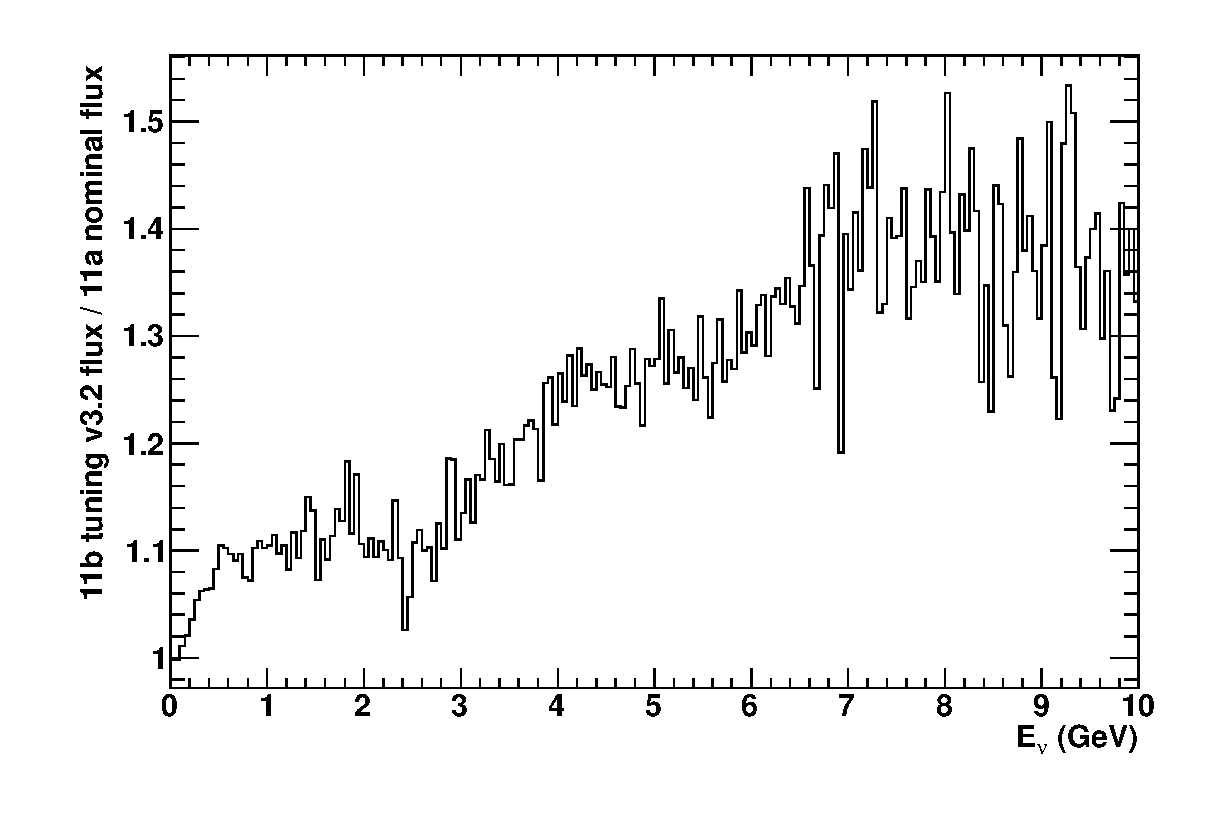
\includegraphics[width=18pc]{./images/fluxtune/fluxtune_numu}
\caption {
  $\nu_\mu$ 2011b\_v3.2\_run1-3c flux tuning weights applied to nominal $\nu_\mu$ and oscillated-$\nu_e$ MC templates.}
\label{fig:na61_weights:numu}
\end{minipage}
\hspace{0.06\linewidth}
\begin{minipage}[t]{0.48\linewidth}
\center
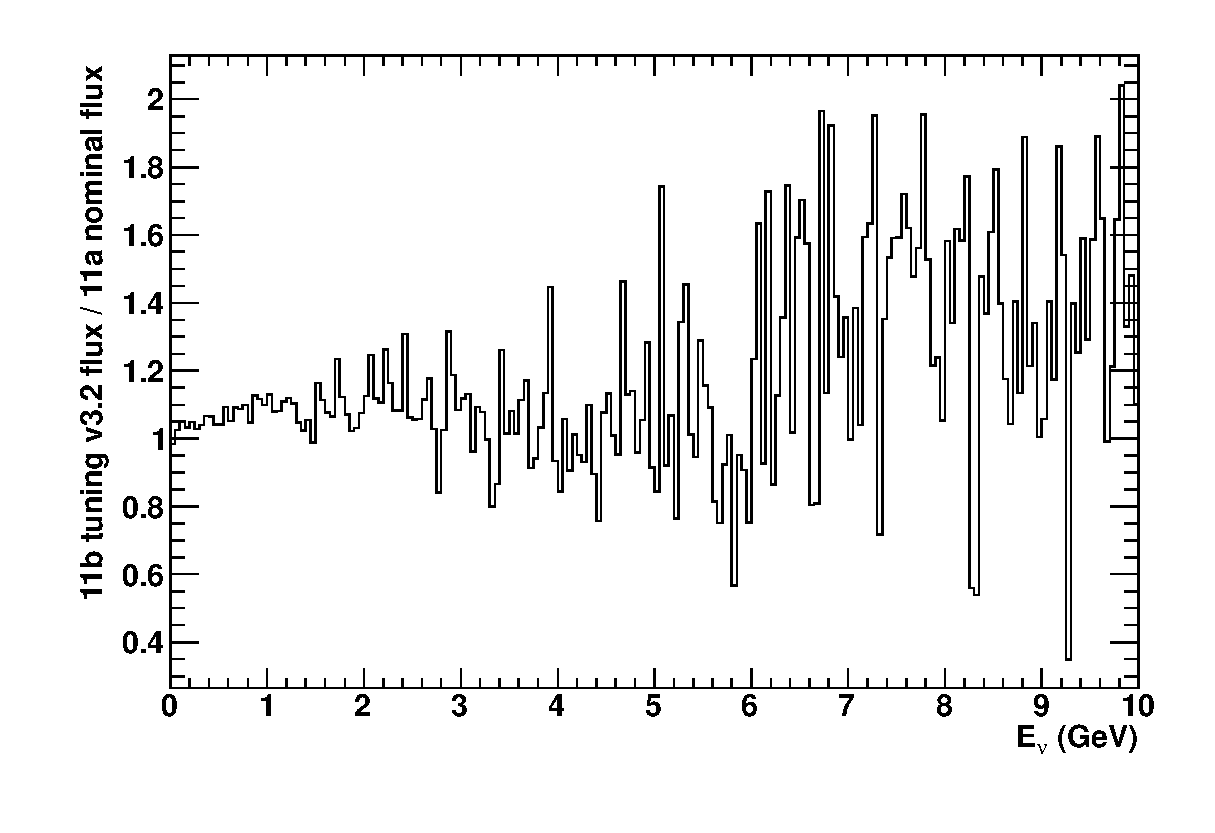
\includegraphics[width=18pc]{./images/fluxtune/fluxtune_numub}
\caption {
  $\bar{\nu_\mu}$ 2011b\_v3.2\_run1-3c flux tuning weights applied to nominal $\bar{\nu_\mu}$ MC templates.}
\label{fig:na61_weights:numubar}
\end{minipage}
\vfill
\begin{minipage}[t]{0.48\linewidth}
\center
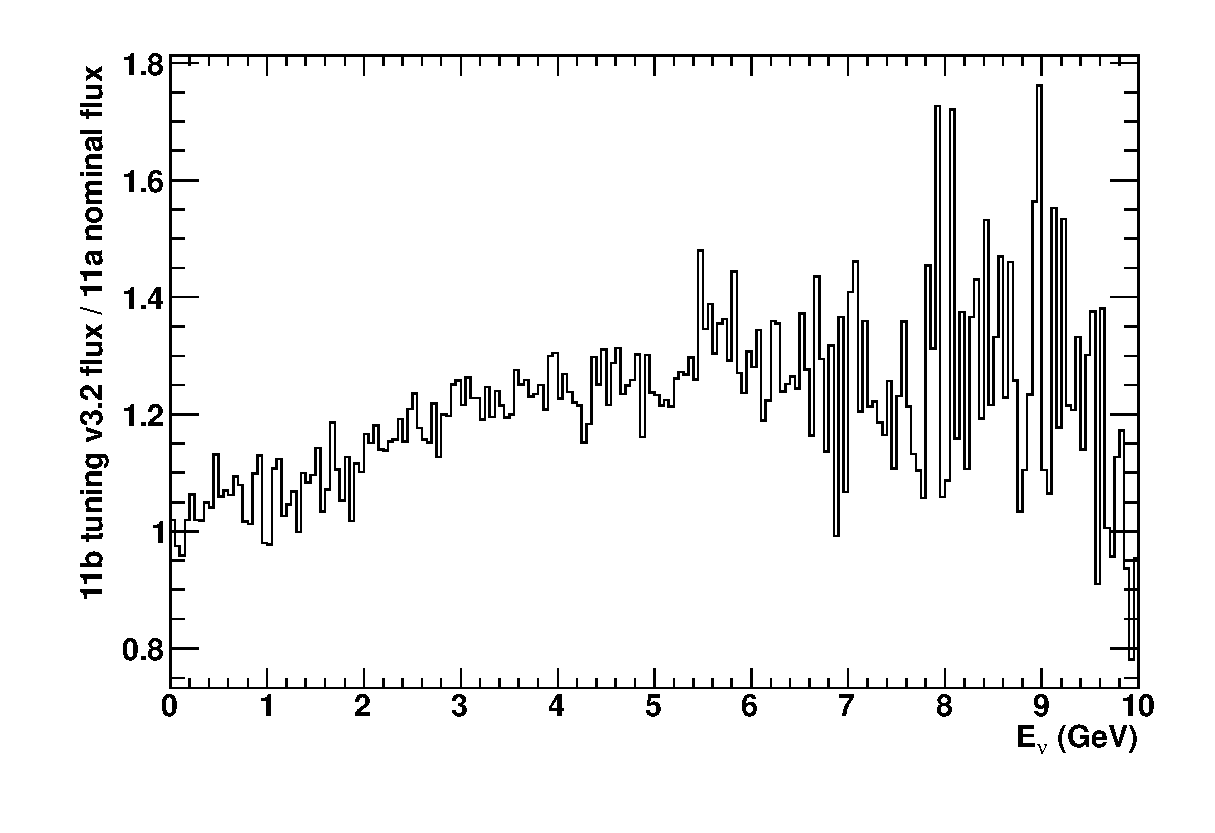
\includegraphics[width=18pc]{./images/fluxtune/fluxtune_nue}
\caption {
  $\nu_e$ 2011b\_v3.2\_run1-3c flux tuning weights applied to nominal $\nu_e$ MC templates.}
\label{fig:na61_weights:nue}
\end{minipage}
\hspace{0.06\linewidth}
\begin{minipage}[t]{0.48\linewidth}
\center
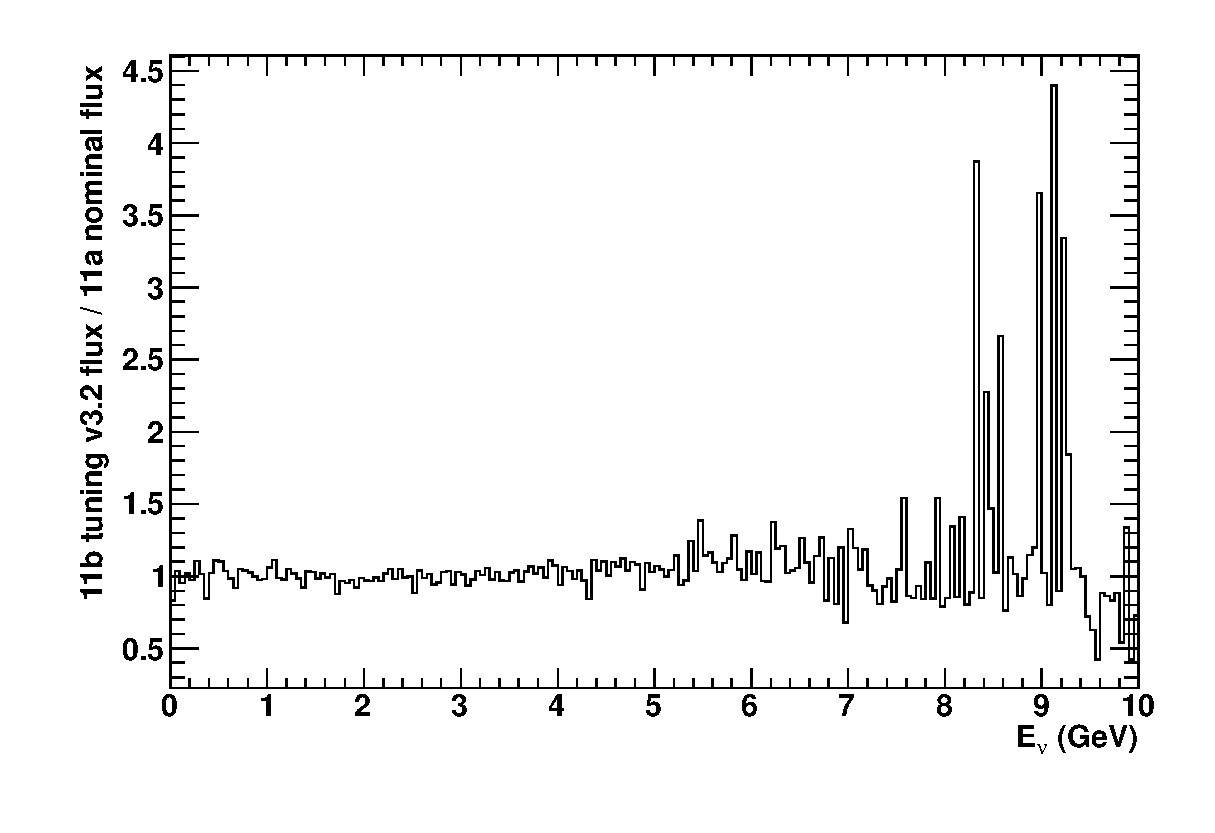
\includegraphics[width=18pc]{./images/fluxtune/fluxtune_nueb}
\caption {
  $\bar{\nu_e}$ 2011b\_v3.2\_run1-3c flux tuning weights applied to nominal $\bar{\nu_e}$ MC templates.}
\label{fig:na61_weights:nuebar}
\end{minipage}
\end{figure*}

%....................................................................................................................
%....................................................................................................................

\subsection {Applying flux and cross-section (BANFF) tuning based on ND280 data}
\label{sec:banff_weights}

This analysis uses the flux and cross-section parameter tuning performed by the 
beam and ND280 flux extrapolation task force (BANFF). 
The BANFF fit combines constraints on the beam flux from the beam monitors and NA61, 
constraints on interaction cross sections from external data (e.g.\ MiniBooNE) and ND280 
measurements of $\nu_\mu$ CCQE-like and CCnonQE-like events with vertices in the FGD fiducial volume.
This fit provides estimates of flux and cross-section parameters 
and their correlations; it also reduces the uncertainties in parameters that are expected to have 
some cancellation between the ND280 and SuperK compared with their uncertainties from external data.
Version 8 of the BANFF fit is used in this analysis \cite{BANFF}.
A list of BANFF parameters and their best-fit values is shown in Tab.\ \ref{tab:banff_params}.

This analysis reweights the NA61-tuned MC templates to the BANFF best-fit parameters
\footnote{
  The BANFF group performed its fit using an NA61-tuned flux ({\em 2011b\_v3.2\_run1-3c}),
  the same one used for reweighting our nominal MC templates in Sec.\ \ref{sec:na61_weights}.
}
\footnote{
  Reweighting the MC templates to the BANFF best-fit parameters is, in effect, a ``special''
  systematic variation. Therefore, more details on 
  are presented in the section detailing the systematic parameters considered in this analysis
  (Sec.\ \ref{sec:systematics}).
}.
The MC templates obtained are referred to, in this document, as the {\em BANFF-tuned} MC templates.
The effect of the BANFF tune on the predicted reconstructed energy spectrum of
single $\mu$-like ring events is discussed in Sec.\ \ref{sec:nominal_and_tuned_predictions} (see 
Figs.\ \ref{fig:nsk_vs_osc_params_effect_of_banff_tune} and \ref{fig:1Rmu_spectrum_w_and_wo_banff_weights}, and
Tabs.\ \ref{tab:nsk_nominal_x3_no_osc} and \ref{tab:nsk_nominal_x3_default_osc}).

%....................................................................................................................
%....................................................................................................................

\subsection{Applying neutrino oscillations}
\label{sec:applying_oscillations}

Oscillation probabilities are computed in a 3-flavour framework including matter effects in constant density matter
(assuming an Earth crust density of 2.6 g/cm$^{3}$).
Custom oscillation probability calculation code was developed within the VaLOR analysis framework.
Details and estimates of the numerical accuracy of this code were first presented in \cite{OurRun12DisappAnalysis3Flavour} 
and, for completeness of the present VaLOR analysis paper, they are given again 
in Appendix \ref{appendix:valor_3f_osc_prob_code}.
Comparisons between the VaLOR oscillation probability calculation code and Prob3++ \cite{Prob3}, 
which is typically used by the alternative T2K oscillation analyses, are shown in Appendix \ref{appendix:comparison_with_prob3}.

Oscillations are applied as a function of true energy to the 
  $\nu_{\mu}$ CCQE,
  $\nu_{\mu}$ CC1$\pi$, 
  $\nu_{\mu}$ CC coherent, 
  $\nu_{\mu}$ CC other, 
  $\bar{\nu}_{\mu}$ CCQE, 
  $\bar{\nu}_{\mu}$ CC1$\pi$, 
  $\bar{\nu}_{\mu}$ CC coherent, 
  $\bar{\nu}_{\mu}$ CC other, 
  $\nu_{e}$ CCQE, 
  $\nu_{e}$ CC1$\pi$,
  $\nu_{e}$ CC coherent,
  $\nu_{e}$ CC other,
  $\bar{\nu}_{e}$ CCQE, 
  $\bar{\nu}_{e}$ CC1$\pi$,
  $\bar{\nu}_{e}$ CC coherent,
  $\bar{\nu}_{e}$ CC other,
  oscillated $\nu_{e}$ CCQE, 
  oscillated $\nu_{e}$ CC1$\pi$,
  oscillated $\nu_{e}$ CC coherent and
  oscillated $\nu_{e}$ CC other
MC templates.

The MC templates constructed from the unoscillated MC samples are weighted 
with the corresponding survival probability:
The $\nu_{\mu}$ templates are weighted with P($\nu_{\mu}\rightarrow\nu_{\mu}$),
the $\bar{\nu}_{\mu}$ templates with P($\bar{\nu}_{\mu}\rightarrow\bar{\nu}_{\mu}$),
the $\nu_{e}$ templates with P($\nu_{e}\rightarrow\nu_{e}$) and
the $\bar{\nu}_{e}$ templates with P($\bar{\nu}_{e}\rightarrow\bar{\nu}_{e}$).
The MC templates made from the oscillated $\nu_{e}$ MC sample are weighted with 
P($\nu_{\mu}\rightarrow\nu_{e}$) (the sample was generated assuming 100\% of 
$\nu_{\mu}$ oscillate to $\nu_{e}$).

We neglect contributions from $\nu_{\tau}$-CC and $\bar{\nu}_{\tau}$-CC as their
energy threshold is around 3.5 GeV and their effect is negligible.

The same $\sin^{2}{2\theta_{23}}$ and $|\Delta m^{2}_{32}|$ parameters 
are used for both $\nu_{\mu}$ and $\bar{\nu_{\mu}}$ oscillations.

Oscillations are not applied to the NC MC templates
  $\nu_{\mu}$ NC1$\pi^{\pm}$, 
  $\nu_{\mu}$ NC other, 
  $\bar{\nu}_{\mu}$ NC1$\pi^{\pm}$, 
  $\bar{\nu}_{\mu}$ NC other, 
  $\nu_{e}$ NC1$\pi^{\pm}$,
  $\nu_{e}$ NC other,
  $\bar{\nu}_{e}$ NC1$\pi^{\pm}$,
  $\bar{\nu}_{e}$ NC other
since, as explained in Sec.\ \ref{sec:mc_templates:template_list}, they serve as proxies for the mixtures of 
$\nu_{e}+\nu_{\mu}+\nu_{\tau}$ NC and 
$\bar{\nu}_{e}+\bar{\nu}_{\mu}+\bar{\nu}_{\tau}$ NC MC templates
which are unchanged under 3-flavour oscillations.


%....................................................................................................................

\subsection {Nominal and tuned-MC single $\mu$-like ring spectrum predictions}
\label{sec:nominal_and_tuned_predictions}

In this section, we present the expected numbers of events and single $\mu$-like ring 
reconstructed energy spectra in SuperK for various oscillation scenarios.
We also present estimates of the effect of the NA61 and BANFF tunings and of assumptions made in the 3-flavour 
neutrino oscillation framework used in this analysis.
Unless explicitly stated otherwise, the normal hierarchy is assumed, 2012 PDG values
are used for $\sin^{2}2\theta_{13}$, $\sin^{2}2\theta_{12}$ and $\Delta m^{2}_{21}$ 
and $\delta_{CP}$=0.
All plots were generated for an integrated exposure of 3.010$\times$10$^{20}$ POT.

The expected number of single $\mu$-like ring events is shown in Fig.\ \ref{fig:nsk_vs_osc_params_tuned_mc}
as a function of the oscillation parameters $\sin^{2}{2\theta_{23}}$ and $|\Delta m^{2}_{32}|$.
The expected number of events ranges from $\sim$58.5
at maximal mixing and at the 2012 MINOS best-fit $|\Delta m^{2}_{32}|$ (2.39$\times10^{-3}$ $eV^{2}/c^{4}$) \cite{MINOS2012},
to more than $\sim$76 for oscillation parameter values still within the 2012 MINOS 90\% confidence region.
This illustrates the great sensitivity of T2K in measuring the $\theta_{23}$ mixing angle.

Predicted single $\mu$-like ring SuperK reconstructed energy spectra are shown in 
Fig. \ref{fig:1Rmu_spectrum_and_components_no_osc} for no oscillations, and in
Fig. \ref{fig:1Rmu_spectrum_and_components_default_osc} for oscillations
with $\sin^{2}2\theta_{23}$ = 1.0 and $|\Delta m^{2}_{32}|$ = 2.4$\times10^{-3}$ $eV^{2}/c^{4}$.

MC tunes derived using NA61 and ND280 data are applied to the nominal MC templates as described earlier 
in this section.
In Fig.\ \ref{fig:nsk_vs_osc_params_effect_of_na61_tune}, the fractional difference is shown in 
the expected number of single $\mu$-like ring events, 
as a function of oscillation parameters $\sin^{2}{2\theta_{23}}$ and $|\Delta m^{2}_{32}|$,
obtained when this analysis switches from the nominal MC to the NA61-tuned MC templates. 
The fractional difference in the expected number of single $\mu$-like ring events 
when switching from the NA61-tuned MC templates to the BANFF-tuned MC templates is also shown in 
Fig. \ref{fig:nsk_vs_osc_params_effect_of_banff_tune}. 
From these figures it can be seen that, for oscillation parameters in the 2012 MINOS 90\% confidence region, 
$\sim$11.5-12.5\% more single $\mu$-like ring events are obtained with
the NA61-tuned MC than with the nominal MC.
In the same part of the parameter space, $\sim$1.8-2.0\% fewer events are expected with the BANFF-tuned MC 
than with the NA61-tuned MC.
The effects of the NA61 and BANFF tunes on the total expected number of single $\mu$-like ring events 
and on the numbers in each of the 28 component reaction modes are shown in 
Tab.\ \ref{tab:nsk_nominal_x3_no_osc} for no oscillations, and in
Tab.\ \ref{tab:nsk_nominal_x3_default_osc} for oscillations
with $\sin^{2}2\theta_{23}$ = 1.0 and $|\Delta m^{2}_{32}|$ = 2.4$\times10^{-3}$ $eV^{2}/c^{4}$.
Finally, the effect of the NA61 and BANFF tunes on the reconstructed energy spectrum of
single $\mu$-like ring events is shown in Figs.\
\ref{fig:1Rmu_spectrum_w_and_wo_na61_weights} and
\ref{fig:1Rmu_spectrum_w_and_wo_banff_weights} respectively. 
In each case, spectra are shown for both no oscillations and for
oscillations with $\sin^{2}2\theta_{23}$ = 1.0 and $|\Delta m^{2}_{32}|$ = 2.4$\times10^{-3}$ $eV^{2}/c^{4}$.

The effect of the choice of octant of $\theta_{23}$ \footnote{
  It should be noted that, in the earlier versions of this note, the first octant ($\sin(\theta) \leq 0.5$) was assumed for all the PMNS oscillation angles. 
In this version, the first octant is assumed for all mixing angles unless explicitly stated otherwise.
The octant choice does however make a difference;
by making some approximations to the 3-flavour P($\nu_{\mu}\rightarrow\nu_{\mu}$) formula % in equation \ref{eq:numusurv3f}. 
%(setting $\Delta m_{32}^{2}$ = $\Delta m_{31}^{2}$, and neglecting $\Delta m_{21}^{2}$ and the third terms in both $|U_{\mu 1}|^{2}$ and $|U_{\mu 2}|^{2}$,
%and assuming vacuum oscillations), %Lorena
(neglecting $\sin^2\left(\frac{\Delta m^2_{21} L}{4E}\right)$ and $\sin^2\left(\frac{2 \Delta m^2_{31} L}{4E}\right)$), %Minamino-san
we get
\begin{equation}
  P(\nu_{\mu}\rightarrow\nu_{\mu})
  \approx 1 - \left( \cos^4(\theta_{13})\sin^2(2\theta_{23}) + \sin^2(\theta_{23})\sin^2(2\theta_{13}) \right) \sin^2\left(\frac{\Delta m_{31}^{2} L}{4E}\right). %Minamino-san
  %\approx 1 - \left( \cos^2(\theta_{13})\sin^2(2\theta_{23}) + \sin^4(\theta_{23})\sin^2(2\theta_{13}) \right) \sin^2\left(\frac{\Delta m_{31}^{2} L}{4E}\right). %Lorena
  \label{eqn:numusurv3fapprox}
\end{equation}
The minimum of Eq.\ \ref{eqn:numusurv3fapprox} occurs at
\begin{equation}
  \sin^2(\theta_{23})
  = \frac{1}{2(1-\sin^2(\theta_{13}))},
  \label{eqn:numusurv3fmin}
\end{equation}
and so, when $\theta_{13} \ne 0$, moves from $\sin^2(\theta_{23}) = 0.5$ to $\sin^2(\theta_{23}) > 0.5$.
More discussion of this effect can be found in Appendix E of \cite{OurRun123JointOscillationAnalysis}.
It should be noted that when $\sin^2(2\theta_{23}) = 1.000$, the oscillation probability is identical,
no matter the value of $\theta_{13}$, and no matter which octant is chosen.
For both $\sin^2(\theta_{12})$ and $\sin^2(\theta_{13})$ we always assume the first octant.
} on the energy spectrum of
single $\mu$-like ring events is shown in Fig.\
\ref{fig:1Rmu_spectrum_octant_comparison}, for oscillations with
$\sin^{2}2\theta_{23}$ = 0.95 (the 2012 PDG 90\% lower limit) and
$|\Delta m^{2}_{32}|$ = 2.4$\times10^{-3}$ $eV^{2}/c^{4}$.
It follows from Eq.\ \ref{eqn:numusurv3fapprox} that the effect of changing from the first to second octant is 
to increase the depth of the oscillation dip, which is why the spectra are almost identical above the oscillation maximum.
The fractional difference in the total expected number of single $\mu$-like ring events when switching between the first and second octant
is shown in Fig.\ \ref{fig:nsk_vs_osc_params_tuned_mc_effect_of_octant}.

When making a fit to obtain the best-fit values of $\sin^{2}2\theta_{23}$ and $|\Delta m^{2}_{32}|$, we fix the 
non-23 oscillation parameters: $\sin^{2}2\theta_{13}$, $\sin^{2}2\theta_{12}$ $\Delta m^{2}_{21}$ are fixed 
to the 2012 PDG values and $\delta_{CP}$ is fixed to 0 (see Sec.\ \ref{sec:oscfit_method_non23params}). The 
maximum possible effect of this assumption on the expected number of single $\mu$-like ring events is shown 
in Fig.\ \ref{fig:nsk_vs_osc_params_tuned_mc_effect_of_non23}.
In each bin of $\sin^{2}{2\theta_{23}}$ and $|\Delta m^{2}_{32}|$,
a large number of toy MC experiments was generated with randomized values of the non-23 parameters. 
The random values of $\sin^{2}2\theta_{13}$, $\sin^{2}2\theta_{12}$ and $\Delta m^{2}_{21}$ were drawn from 
Gaussian distributions with means equal to the 2012 PDG values and standard deviations equal to the 1$\sigma$ 
errors, while the values of $\delta_{CP}$ were drawn from a uniform distribution between -$\pi$ and +$\pi$.
These four non-23 parameters were taken to be uncorrelated.
The maximum frational deviation from the default case was recorded and plotted 
in Fig.\ \ref{fig:nsk_vs_osc_params_tuned_mc_effect_of_non23}.
From this figure, it can be seen that the effect of the non-23-sector oscillation parameters is small:
the maximum fractional deviation from the default assumption is of the order of $\sim$1\% in the part of 
the parameter space covered by the 2012 MINOS 90\% confidence region. 

All the results in this analysis assume the normal mass hierarchy. 
The effect of this assumption on the expected number of single $\mu$-like ring events
is shown in Fig.\ \ref{fig:nsk_vs_osc_params_tuned_mc_effect_of_hierarchy} 
as a function of the oscillation parameters $\sin^{2}{2\theta_{23}}$ and $|\Delta m^{2}_{32}|$.
The effect is large and potentially misleading, and some clarifications are in order.
This analysis can assume a given hierarchy (in our case, normal) without loss of generality of its results.
Fig.\ \ref{fig:nsk_vs_osc_params_tuned_mc_effect_of_hierarchy} reveals that $|\Delta m^{2}_{32}|$ is a poor 
choice as the atmospheric mass-squared difference when both mass hierarchies need to be considered,
since $|\Delta m^{2}_{32}|$ is the largest mass-squared difference for the inverted hierarchy 
but the second-largest for the normal hierarchy. 
The large difference shown in Fig.\ \ref{fig:nsk_vs_osc_params_tuned_mc_effect_of_hierarchy} 
is caused by the change in value of $\Delta m^{2}_{31}$ when switching from the
normal to inverted hierarchy.

Other choices exist for the atmospheric mass-squared difference, and these are explained in Sec.\ 
\ref{sec:oscfit_method_23param_choice}. An example of an alternative choice is shown vividly in 
Fig.\ 5 in \cite{OurRun12DisappAnalysis3Flavour}; this technical note describes a repeat, in a 3-flavour 
framework, of our official Run1+2 disappearance analysis \cite{OurRun12DisappAnalysis} which was originally 
performed in a 2-flavour framework.

The reader may also be interested in comparisons of oscillated single $\mu$-like ring spectra,
obtained in a 3-flavour framework with spectra obtained in a 2-flavour framework.
Many such comparisons were presented in \cite{OurRun12DisappAnalysis3Flavour}.

%...........
%
% nsk
%
\begin{figure*}[htb]
\center
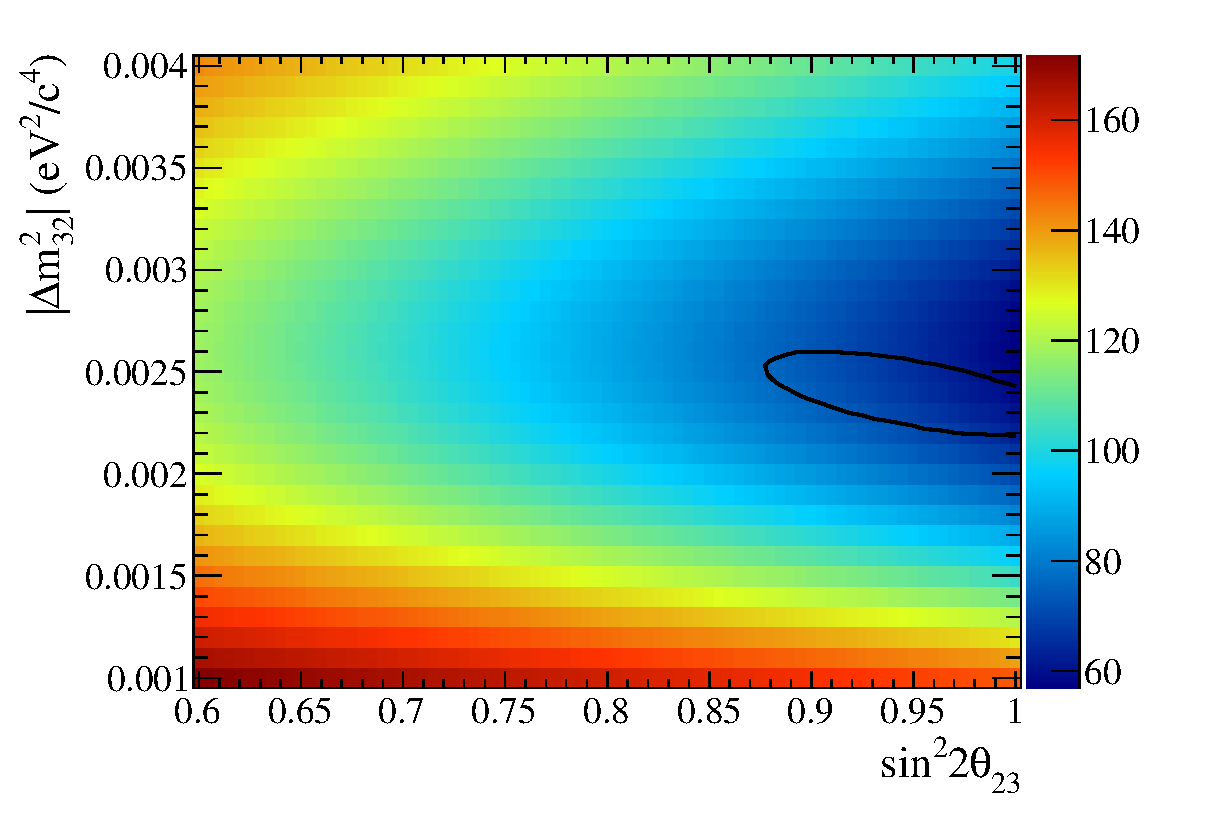
\includegraphics[width=32pc]{./images/spectrum_nominal/nsk_nominalbanff}
\caption {
  Predicted number of 1-ring $\mu$-like events,
  as a function of $\sin^{2}2\theta_{23}$ and $|\Delta m^{2}_{32}|$,
  for an exposure of 3.010$\times$10$^{20}$ POT.
  The number of events was calculated using the BANFF-tuned MC templates.
  2012 PDG values are used for $\sin^{2}2\theta_{13}$, $\sin^{2}2\theta_{12}$ and $\Delta m^{2}_{21}$ and $\delta_{CP}$=0. 
  The numbers shown were generated assuming the normal hierarchy.
  The 2012 MINOS 90\% confidence region is superimposed for reference.
}
\label{fig:nsk_vs_osc_params_tuned_mc}
\end{figure*}

%...........
%
% spectra, various osc scenarios
%
\begin{figure*}[htb]
\begin{minipage}[t]{0.48\linewidth}
\center
\includegraphics[width=20pc]{{./images/spectrum_nominal/sk_ereco_spectrum-0.000000-0.000000-grouped-components}.eps}
\caption {
Predicted reconstructed-energy spectrum of 1-ring $\mu$-like events,
and contributions from various true neutrino reaction modes,
for no oscillations and
for an exposure of 3.010$\times$10$^{20}$ POT.
The 28 components of the spectrum are calculated separately in the actual analysis, 
but, for this plot, are grouped into just 5 categories: 
$\nu_{\mu}$ CCQE, $\nu_{\mu}$ CCnonQE, $\bar{\nu_{\mu}}$ CC, $\nu_{e}$/$\bar{\nu_{e}}$ CC and NC.
The spectrum was generated using the BANFF-tuned MC templates.
}
\label{fig:1Rmu_spectrum_and_components_no_osc}
\end{minipage}
\hspace{0.06\linewidth}
\begin{minipage}[t]{0.48\linewidth}
\center
\includegraphics[width=20pc]{{./images/spectrum_nominal/sk_ereco_spectrum-1.000000-0.002400-grouped-components}.eps}
\caption {
Predicted reconstructed-energy spectrum of 1-ring $\mu$-like events,
and contributions from various true neutrino reaction modes,
for oscillations with $\sin^{2}2\theta_{23}$=1.0 and $|\Delta m^{2}_{32}|$=2.4$\times10^{-3}$ $eV^{2}/c^{4}$ 
and for an exposure of 3.010$\times$10$^{20}$ POT.
The spectrum was generated using the BANFF-tuned MC templates.
2012 PDG values are used for $\sin^{2}2\theta_{13}$, $\sin^{2}2\theta_{12}$ and $\Delta m^{2}_{21}$ and $\delta_{CP}$=0. 
The spectrum shown was generated assuming the normal hierarchy.
Note that the vertical axis is zoomed in by a factor of 4 compared with Fig.\ \ref{fig:1Rmu_spectrum_and_components_no_osc}.
}
\label{fig:1Rmu_spectrum_and_components_default_osc}
\end{minipage}
\end{figure*}

%...........
%
% effect of tunes on nsk
%
\begin{figure*}[htb]
\begin{minipage}[t]{0.48\linewidth}
\center
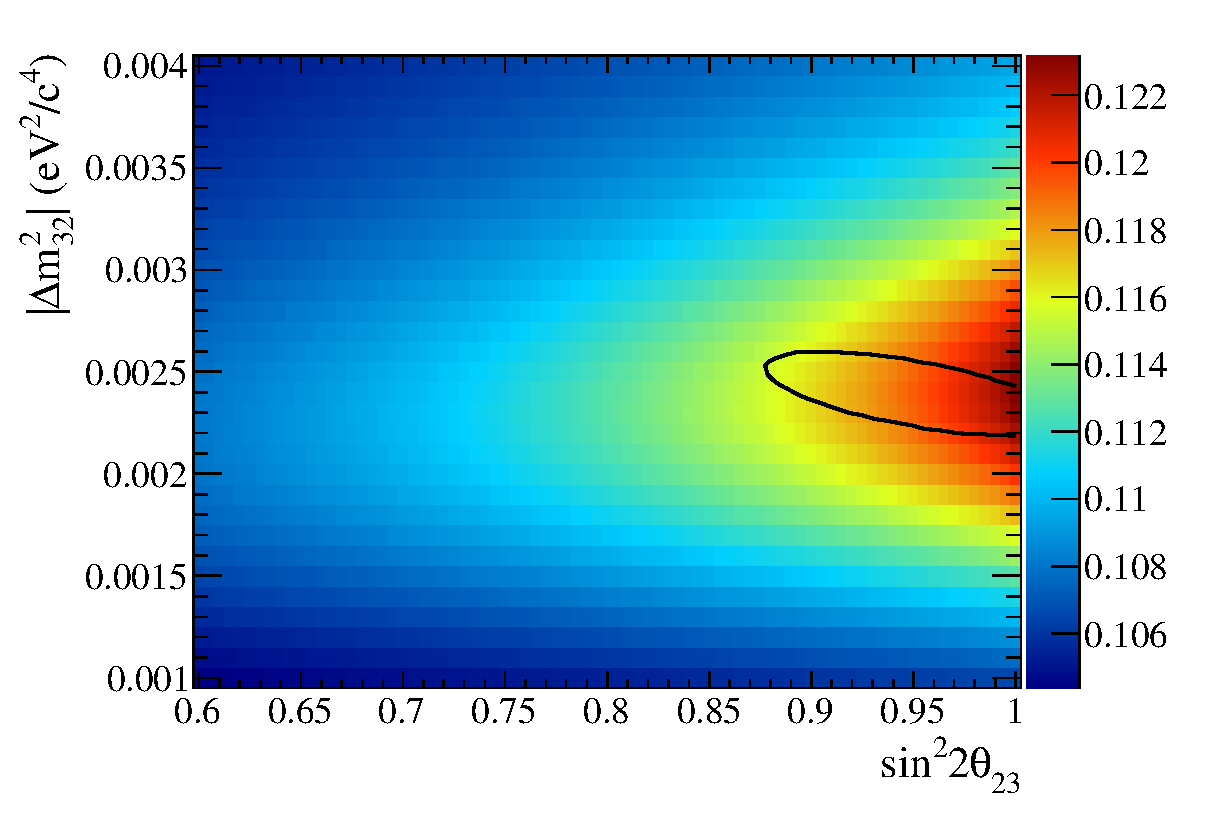
\includegraphics[width=18pc]{./images/spectrum_nominal/nsk_diff_nomflux}
\caption {
  Fractional difference in the predicted number of 1-ring $\mu$-like events 
  as a result of applying the 2011b v3.2 flux tuning to the nominal MC templates.
  This number is shown as a function of $\sin^{2}2\theta_{23}$ and $|\Delta m^{2}_{32}|$
  for an exposure of 3.010$\times$10$^{20}$ POT.
  The 2012 PDG parameters are used for $\sin^{2}2\theta_{13}$, $\sin^{2}2\theta_{12}$ and $\Delta m^{2}_{21}$,and $\delta_{CP}$=0. 
  The numbers shown were generated assuming the normal hierarchy.
  The MINOS 2012 90\% CL region is superimposed for reference.
}
\label{fig:nsk_vs_osc_params_effect_of_na61_tune}
\end{minipage}
\hspace{0.06\linewidth}
\begin{minipage}[t]{0.48\linewidth}
\center
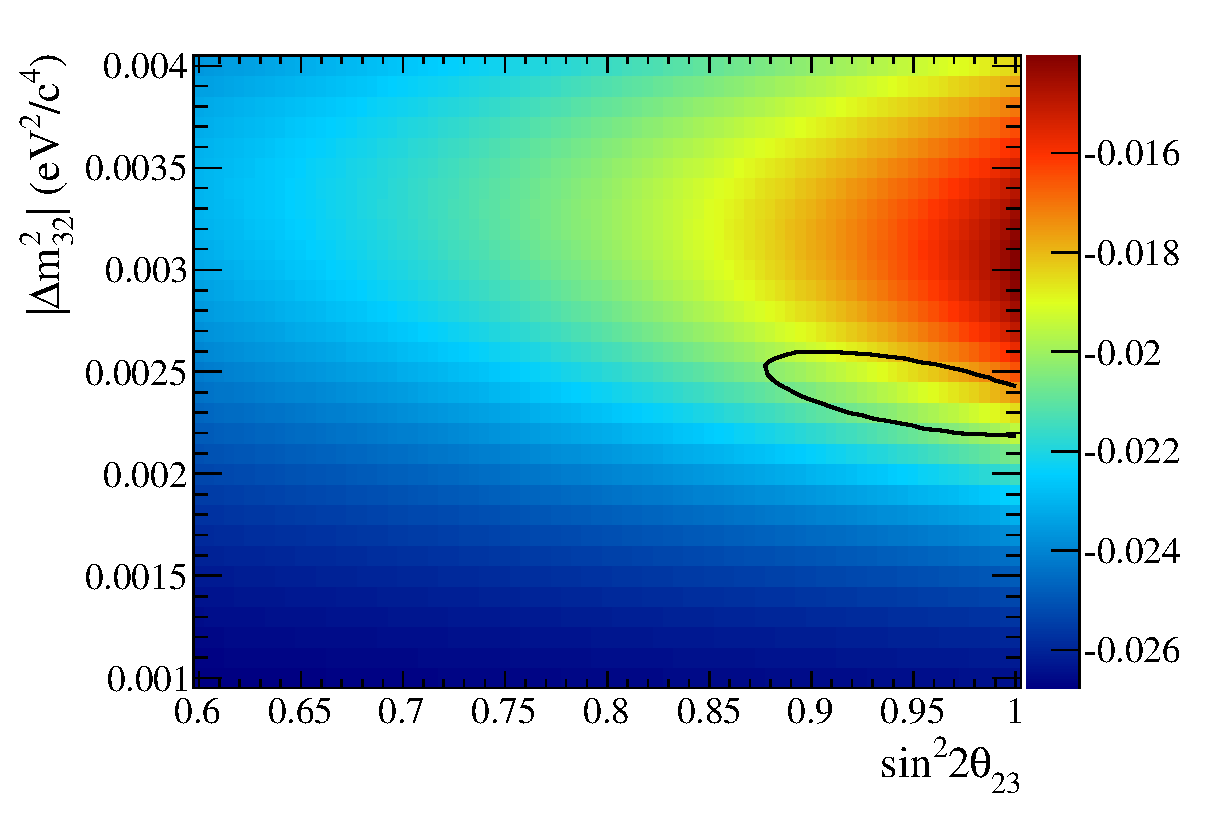
\includegraphics[width=18pc]{./images/spectrum_nominal/nsk_diff_tunflux}
\caption {
  Fractional difference in the predicted number of 1-ring $\mu$-like events
  as a result of applying the BANFF flux and cross-section tuning to the 2011b v3.2 flux tuned MC templates.
  This number is shown as a function of $\sin^{2}2\theta_{23}$ and $|\Delta m^{2}_{32}|$ and 
  for an exposure of 3.010$\times$10$^{20}$ POT.
  The 2012 PDG values are used for $\sin^{2}2\theta_{13}$, $\sin^{2}2\theta_{12}$ and $\Delta m^{2}_{21}$, and $\delta_{CP}$=0. 
  The numbers shown were generated assuming the normal hierarchy.
  The MINOS 2012 90\% CL region is superimposed for reference.
}
\label{fig:nsk_vs_osc_params_effect_of_banff_tune}
\end{minipage}
\end{figure*}


%...........
%
% tables showing the effect of tunes on nsk and nsk components
%
\begin{table}
\centering
\begin{tabular}{| c | c | c | c | }
\hline
       & $N_{SK}$     & $N_{SK}$         & $N_{SK}$                      \\
       & (nominal MC) & (NA61-tuned MC)  & (BANFF-tuned MC)  \\
\hline
Total & 190.986142 & 210.464599 &  204.747590 \\
\hline
$\nu_\mu$ CCQE &      151.820154 & 166.353705 & 155.044970 \\
$\nu_\mu$ CC 1$\pi$ &       25.717606 & 28.879686 & 34.945661 \\
$\nu_\mu$ CC coherent &        0.898432 & 1.005621 & 0.950276 \\
$\nu_\mu$ CC other &        3.584984 & 4.315475 & 4.198557 \\
$\nu_\mu$/$\nu_\tau$ NC 1$\pi^{+/-}$ &        1.492903 & 1.696744 & 1.625483 \\
$\nu_\mu$/$\nu_\tau$ NC other &        1.294522 & 1.521644 & 1.466497 \\
$\bar{\nu}_{\mu}$ CCQE &        4.118572 & 4.459811 & 3.981437 \\
$\bar{\nu}_{\mu}$ CC 1$\pi$ &        1.336699 & 1.445418 & 1.762408 \\
$\bar{\nu}_{\mu}$ CC coherent &        0.194978 & 0.211123 & 0.202799 \\
$\bar{\nu}_{\mu}$ CC other &        0.236537 & 0.253912 & 0.247794 \\
$\bar{\nu}_{\mu}$/$\bar{\nu}_{\tau}$ NC 1$\pi^{+/-}$ &        0.084582 & 0.091984 & 0.090422 \\
$\bar{\nu}_{\mu}$/$\bar{\nu}_{\tau}$ NC other &        0.073460 & 0.079580 & 0.077614 \\
$\nu_e$ CCQE &        0.015774 & 0.016972 & 0.016260 \\
$\nu_e$ CC 1$\pi$ &        0.009050 & 0.009932 & 0.013125 \\
$\nu_e$ CC coherent &        0.000403 & 0.000434 & 0.000434 \\
$\nu_e$ CC other &        0.002568 & 0.003048 & 0.003051 \\
$\nu_e$ NC 1$\pi^{+/-}$ &        0.042494 & 0.048652 & 0.049421 \\
$\nu_e$ NC other &        0.049084 & 0.057414 & 0.057684 \\
$\bar{\nu}_{e}$ CCQE &        0.000822 & 0.000827 & 0.000790 \\
$\bar{\nu}_{e}$ CC 1$\pi$ &        0.000599 & 0.000601 & 0.000745 \\
$\bar{\nu}_{e}$ CC coherent &        0.000073 & 0.000073 & 0.000073 \\
$\bar{\nu}_{e}$ CC other &        0.000214 & 0.000219 & 0.000219 \\
$\bar{\nu}_{e}$ NC 1$\pi^{+/-}$ &        0.005755 & 0.005805 & 0.005916 \\
$\bar{\nu}_{e}$ NC other &        0.005876 & 0.005918 & 0.005954 \\
Oscillated $\nu_e$ CCQE &        0.000000 & 0.000000 & 0.000000 \\
Oscillated $\nu_e$ CC 1$\pi$ &        0.000000 & 0.000000 & 0.000000 \\
Oscillated $\nu_e$ CC coherent &        0.000000 & 0.000000 & 0.000000 \\
Oscillated $\nu_e$ CC other &        0.000000 & 0.000000 & 0.000000 \\
\hline
\end{tabular}
\caption{
  Calculated numbers of 1-ring $\mu$-like events without oscillations using the nominal MC templates, the 
  NA61-tuned MC templates and the BANFF-tuned MC templates.
  The total numbers of events and the numbers of events from each mode considered in this analysis are shown.
  These numbers were calculated for an exposure of 3.010$\times$10$^{20}$ POT.
}
\label{tab:nsk_nominal_x3_no_osc}
\end{table}


\begin{table}
\centering
\begin{tabular}{| c | c | c | c | }
\hline
       & $N_{SK}$     & $N_{SK}$              & $N_{SK}$                      \\
       & (nominal MC) & (NA61-tuned MC)  & (BANFF-tuned MC)  \\
\hline
Total & 52.890886 & 59.406174 & 58.367775 \\
\hline
$\nu_\mu$ CCQE &       30.122383 & 33.277415 & 30.285520 \\
$\nu_\mu$ CC 1$\pi$ &       12.736216 & 14.628739 & 16.931486 \\
$\nu_\mu$ CC coherent &        0.365047 & 0.420613 & 0.399710 \\
$\nu_\mu$ CC other &        3.187277 & 3.862403 & 3.771051 \\
$\nu_\mu$/$\nu_\tau$ NC 1$\pi^{+/-}$ &        1.492903 & 1.696744 & 1.625483 \\
$\nu_\mu$/$\nu_\tau$ NC other &        1.294522 & 1.521644 & 1.466497 \\
$\bar{\nu}_{\mu}$ CCQE &        2.023300 & 2.190691 & 1.891082 \\
$\bar{\nu}_{\mu}$ CC 1$\pi$ &        0.958303 & 1.032827 & 1.228001 \\
$\bar{\nu}_{\mu}$ CC coherent &        0.104487 & 0.112894 & 0.108444 \\
$\bar{\nu}_{\mu}$ CC other &        0.209999 & 0.225107 & 0.220043 \\
$\bar{\nu}_{\mu}$/$\bar{\nu}_{\tau}$ NC 1$\pi^{+/-}$ &        0.084582 & 0.091984 & 0.090422 \\
$\bar{\nu}_{\mu}$/$\bar{\nu}_{\tau}$ NC other &        0.073460 & 0.079580 & 0.077614 \\
$\nu_e$ CCQE &        0.014633 & 0.015752 & 0.015068 \\
$\nu_e$ CC 1$\pi$ &        0.008572 & 0.009421 & 0.012426 \\
$\nu_e$ CC coherent &        0.000375 & 0.000404 & 0.000404 \\
$\nu_e$ CC other &        0.002530 & 0.003005 & 0.003007 \\
$\nu_e$ NC 1$\pi^{+/-}$ &        0.042494 & 0.048652 & 0.049421 \\
$\nu_e$ NC other &        0.049084 & 0.057414 & 0.057684 \\
$\bar{\nu}_{e}$ CCQE &        0.000785 & 0.000790 & 0.000755 \\
$\bar{\nu}_{e}$ CC 1$\pi$ &        0.000583 & 0.000585 & 0.000724 \\
$\bar{\nu}_{e}$ CC coherent &        0.000070 & 0.000070 & 0.000070 \\
$\bar{\nu}_{e}$ CC other &        0.000212 & 0.000217 & 0.000217 \\
$\bar{\nu}_{e}$ NC 1$\pi^{+/-}$ &        0.005755 & 0.005805 & 0.005916 \\
$\bar{\nu}_{e}$ NC other &        0.005876 & 0.005918 & 0.005954 \\
Oscillated $\nu_e$ CCQE &        0.079970 & 0.087419 & 0.082883 \\
Oscillated $\nu_e$ CC 1$\pi$ &        0.024965 & 0.027318 & 0.035271 \\
Oscillated $\nu_e$ CC coherent &        0.001860 & 0.002039 & 0.001949 \\
Oscillated $\nu_e$ CC other &        0.000644 & 0.000723 & 0.000672 \\
\hline
\end{tabular}
\caption{
  Calculated numbers of 1-ring $\mu$-like events using the nominal MC templates, the NA61-tuned MC templates
  and the BANFF-tuned MC templates.
  The total numbers of events and the numbers of events from each mode considered in this analysis are shown.
  These numbers were calculated for an exposure of 3.010$\times$10$^{20}$ POT
  and oscillations with $\sin^{2}2\theta_{23}$=1.0 and $|\Delta m^{2}_{32}|$=2.4$\times10^{-3}$ $eV^{2}/c^{4}$.
  The 2012 PDG parameters are used for $\sin^{2}2\theta_{13}$, $\sin^{2}2\theta_{12}$ and $\Delta m^{2}_{21}$ and $\delta_{CP}$=0. 
  The normal hierarchy is assumed.
}
\label{tab:nsk_nominal_x3_default_osc}
\end{table}

%...........
%
% Plots showing the effect of tunes on Ereco spectra
%
\begin{figure*}[htb]
\center
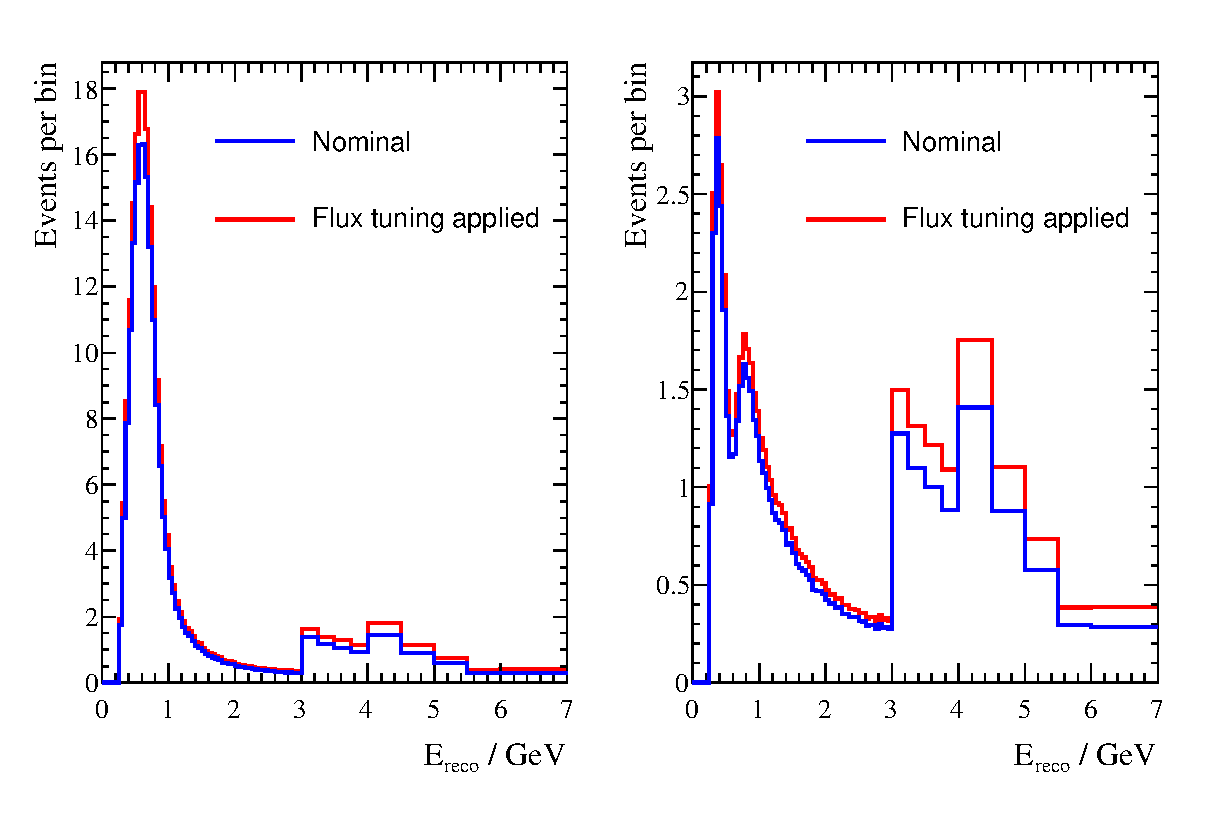
\includegraphics[width=30pc]{./images/spectrum_nominal/spectra_nom_fluxtuned}
\caption {
Reconstructed-energy spectrum of 1-ring $\mu$-like events, 
for an exposure of 3.010$\times$10$^{20}$ POT,
both with and without the effect of the {\em 2011b\_v3.2\_run1-3c} flux tuning of the nominal MC templates. 
The spectra are shown both for no oscillations (left) 
and for oscillations with $\sin^{2}2\theta_{23}$=1.0, $|\Delta m^{2}_{32}|$=2.4$\times10^{-3}$ $eV^{2}/c^{4}$, 
the 2012 PDG values for $\sin^{2}2\theta_{13}$, $\sin^{2}2\theta_{12}$ and $\Delta m^{2}_{21}$, and 
$\delta_{CP}$=0 (right). Results shown for the normal hierarchy.
}
\label{fig:1Rmu_spectrum_w_and_wo_na61_weights}
\end{figure*}

\begin{figure*}[htb]
\center
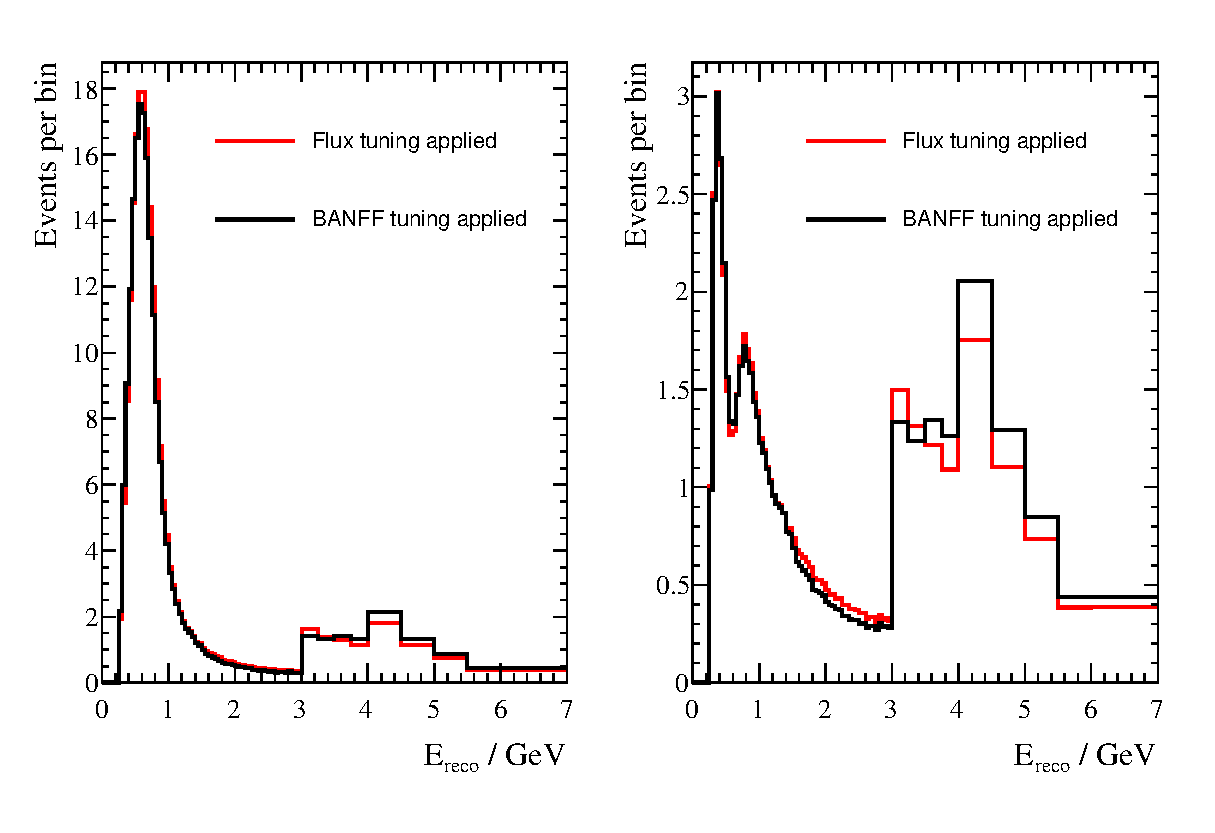
\includegraphics[width=30pc]{./images/spectrum_nominal/spectra_tun_banfftuned}
\caption {
Reconstructed-energy spectrum of 1-ring $\mu$-like events,
for an exposure of 3.010$\times$10$^{20}$ POT,
both with and without the effect of BANFF flux and cross-section tuning on the NA61-tuned {\em 2011b\_v3.2\_run1-3c} flux MC templates.
The spectra are shown both for no 23-sector oscillations (left) 
and for oscillations with $\sin^{2}2\theta_{23}$=1.0 and $|\Delta m^{2}_{32}|$=2.4$\times10^{-3}$ $eV^{2}/c^{4}$ (right).
In all spectra, the 2012 PDG parameters are used for $\sin^{2}2\theta_{13}$, $\sin^{2}2\theta_{12}$ and $\Delta m^{2}_{21}$
and $\delta_{CP}$=0. Results shown for the normal hierarchy.
}
\label{fig:1Rmu_spectrum_w_and_wo_banff_weights}
\end{figure*}

% ...........
%
% effect of octant on spectrum
% effect of octant on Nsk
%
\begin{figure*}[htb]
\begin{minipage}[t]{0.48\linewidth}
\center
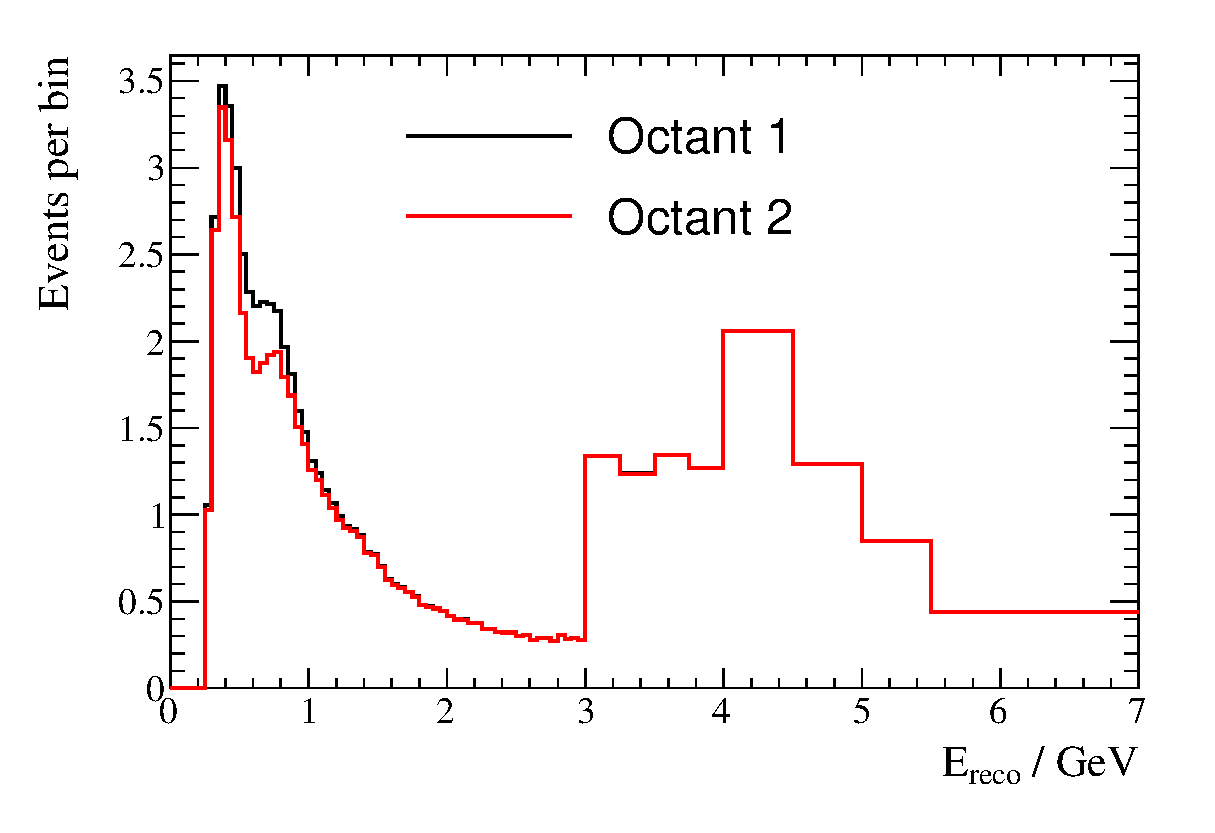
\includegraphics[width=18pc]{./images/spectrum_nominal/spectra_octants}
\caption {
  Predicted reconstructed-energy spectrum of 1-ring $\mu$-like events, 
  for an exposure of 3.010$\times$10$^{20}$ POT,
  for $\theta_{23}$ both in the first octant and second octant. 
  The spectra are shown oscillations with $\sin^{2}2\theta_{23}$=0.95, $|\Delta m^{2}_{32}|$=2.4$\times10^{-3}$ $eV^{2}/c^{4}$, 
  the 2012 PDG values for $\sin^{2}2\theta_{13}$, $\sin^{2}2\theta_{12}$ and $\Delta m^{2}_{21}$, and 
  $\delta_{CP}$=0 (right). Results shown for the normal hierarchy.
}
\label{fig:1Rmu_spectrum_octant_comparison}
\end{minipage}
\hspace{0.06\linewidth}
\begin{minipage}[t]{0.48\linewidth}
\center
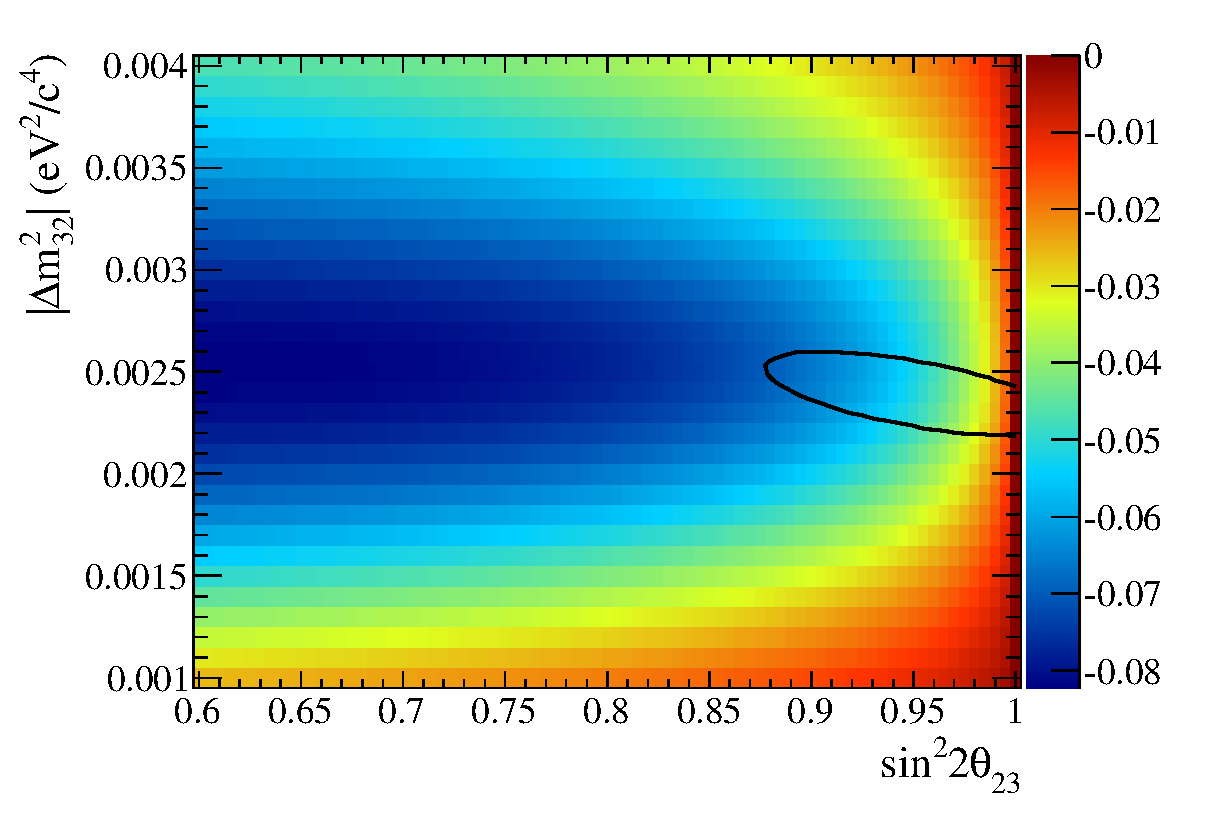
\includegraphics[width=18pc]{./images/spectrum_nominal/nsk_diff_octant}
\caption {
  Fractional difference in the predicted number of 1-ring $\mu$-like events between assuming that $\theta_{23}$ is in the first octant
  and assuming it is in the second octant.
  The fractional difference is shown as function of $\sin^{2}2\theta_{23}$ and $|\Delta m^{2}_{32}|$,
  for an exposure of 3.010$\times$10$^{20}$ POT.
  The number of events was calculated using the BANFF-tuned MC templates.
  The 2012 PDG values are used for $\sin^{2}2\theta_{13}$, $\sin^{2}2\theta_{12}$ and $\Delta m^{2}_{21}$, and $\delta_{CP}$=0.
  Results shown for the normal hierarchy.
  The 2012 MINOS 90\% confidence region is superimposed for reference.
}
\label{fig:nsk_vs_osc_params_tuned_mc_effect_of_octant}
\end{minipage}
\end{figure*}

%...........
%
% Effect of non-23 sector params 
% Effect of mass hierarchy
%
\begin{figure*}[htb]
\begin{minipage}[t]{0.48\linewidth}
\center
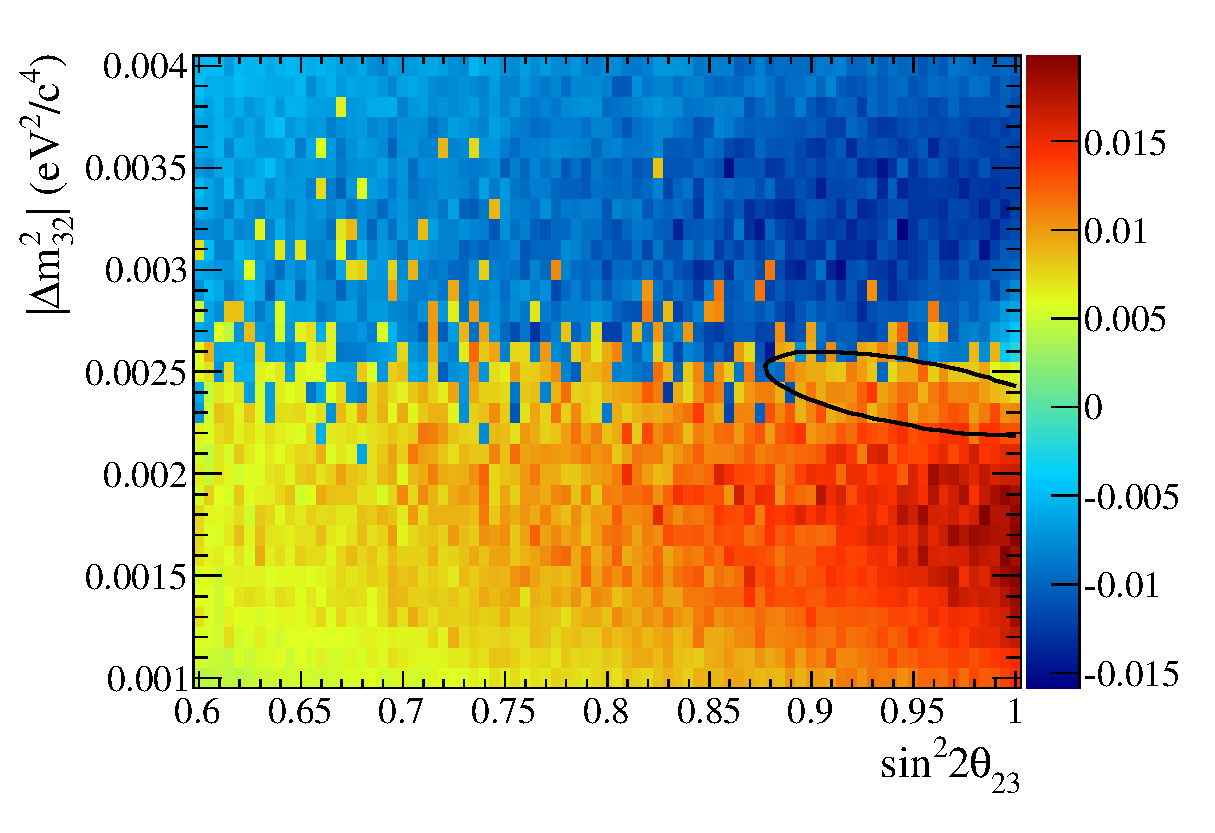
\includegraphics[width=18pc]{./images/spectrum_nominal/nsk_diff_non23throw}
\caption {
  Maximum value of the fractional difference in the predicted number of 1-ring $\mu$-like events
  between varying each of $\sin^{2}2\theta_{13}$, $\sin^{2}2\theta_{12}$, $\Delta m^{2}_{21}$ and $\delta_{CP}$ 
  within their allowed ranges and their nominal values (these are the 2012 PDG values for $\sin^{2}2\theta_{13}$, 
  $\sin^{2}2\theta_{12}$ and $\Delta m^{2}_{21}$, and $\delta_{CP}$=0).
  The fractional difference is shown as function of $\sin^{2}2\theta_{23}$ and $|\Delta m^{2}_{32}|$,
  for an exposure of 3.010$\times$10$^{20}$ POT.
  The number of events was calculated using the BANFF-tuned MC templates.
  The normal hierarchy was assumed.
  The 2012 MINOS 90\% confidence region is superimposed for reference.
}
\label{fig:nsk_vs_osc_params_tuned_mc_effect_of_non23}
\end{minipage}
\hspace{0.06\linewidth}
\begin{minipage}[t]{0.48\linewidth}
\center
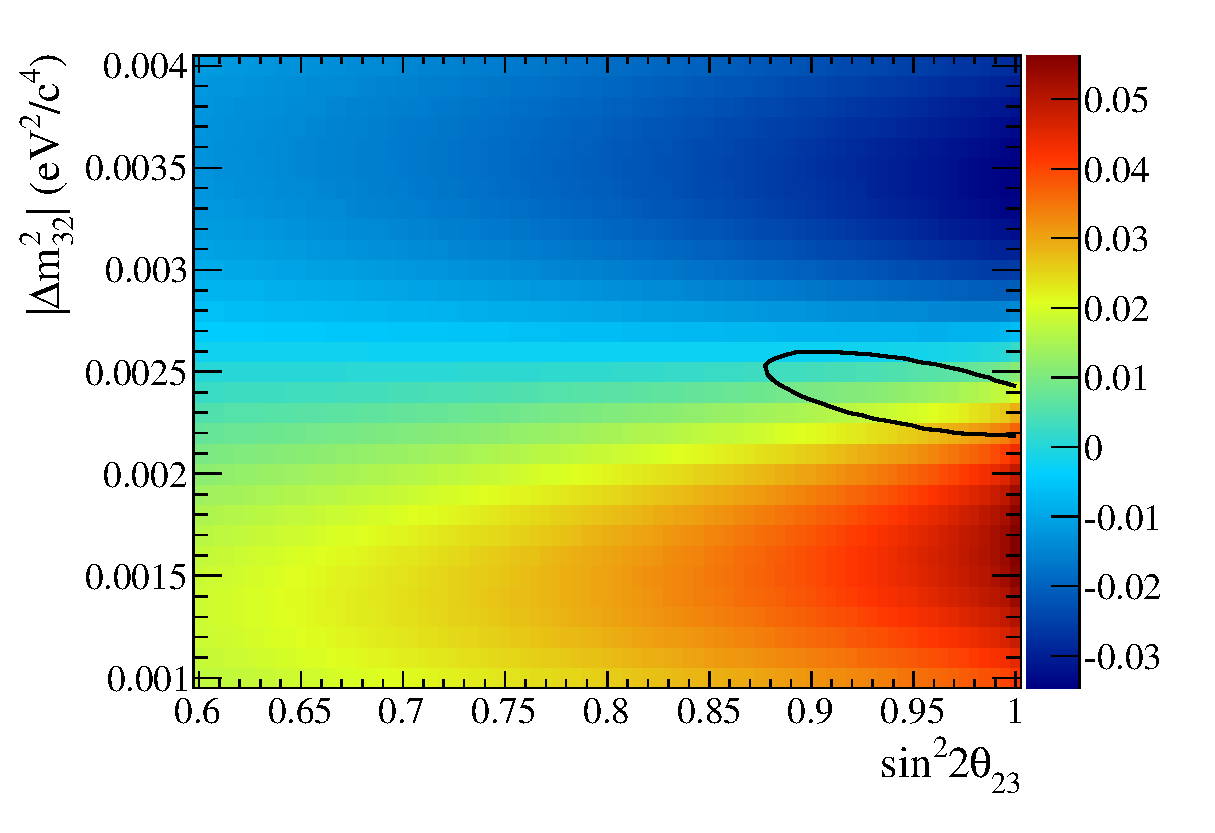
\includegraphics[width=18pc]{./images/spectrum_nominal/nsk_diff_inv}
\caption {
  Fractional difference in the predicted number of 1-ring $\mu$-like events between assuming the normal hierarchy 
  and assuming the inverted hierarchy.
  The fractional difference is shown as function of $\sin^{2}2\theta_{23}$ and $|\Delta m^{2}_{32}|$,
  for an exposure of 3.010$\times$10$^{20}$ POT.
  The number of events was calculated using the BANFF-tuned MC templates.
  The 2012 PDG values are used for $\sin^{2}2\theta_{13}$, $\sin^{2}2\theta_{12}$ and $\Delta m^{2}_{21}$, and $\delta_{CP}$=0. 
  The 2012 MINOS 90\% confidence region is superimposed for reference.
}
\label{fig:nsk_vs_osc_params_tuned_mc_effect_of_hierarchy}
\end{minipage}
\end{figure*}
